\todo{Brief paragraph summarizing what are we going to study
Description of the experimental platform HW OS Compilers,
OpenBLAS
} 

\begin{figure*}[h]
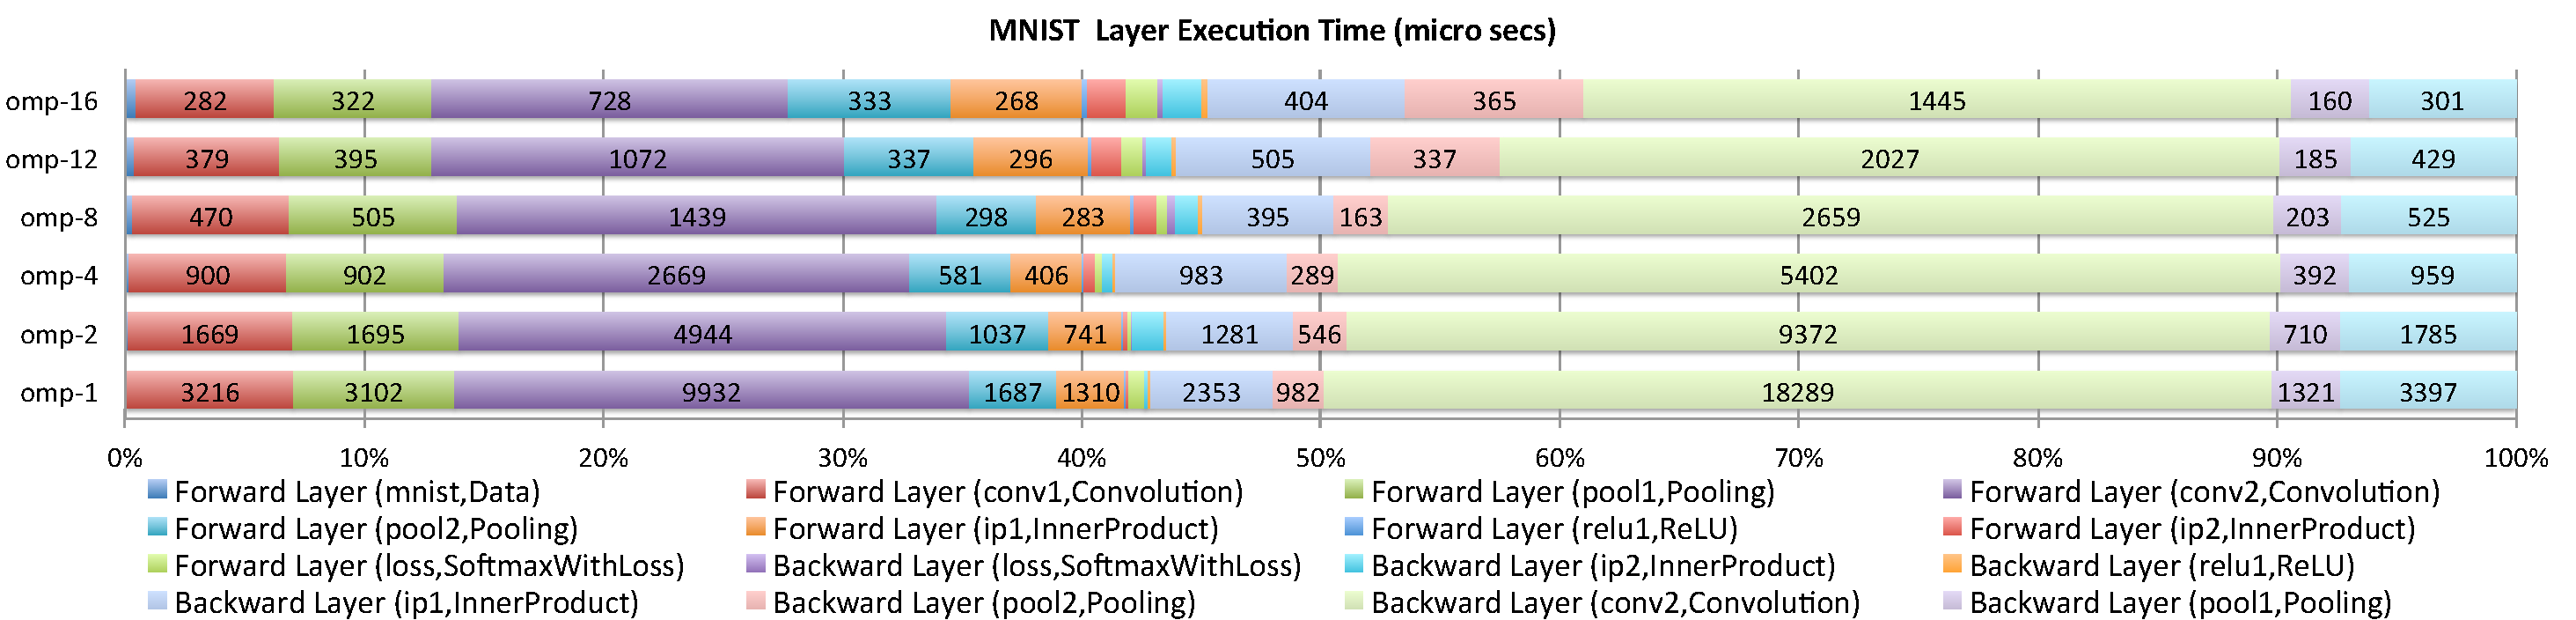
\includegraphics[width=\linewidth]{figures/mnist-rel-abs-time.pdf}
\caption{\todo{CAPTION}}
\end{figure*}

\begin{figure*}[h]
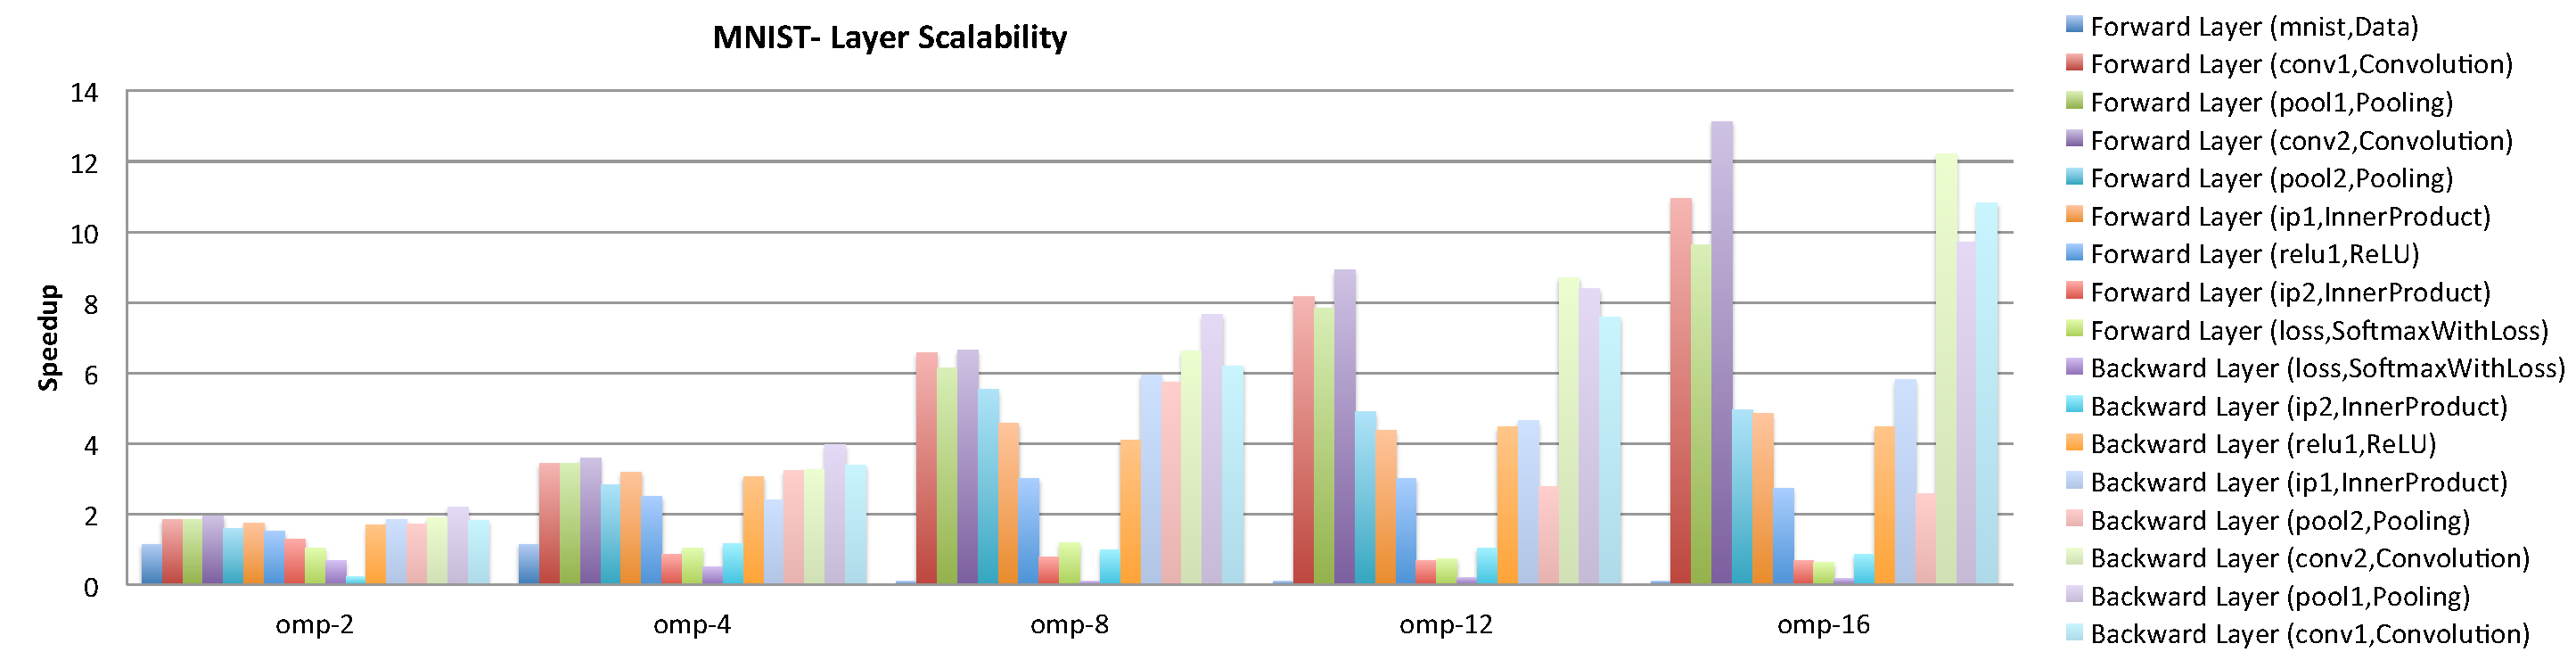
\includegraphics[width=\textwidth]{figures/mnist-scalability-layer.pdf}
\caption{MNIST - Layer Scalability}
\end{figure*}

\begin{figure}[b]
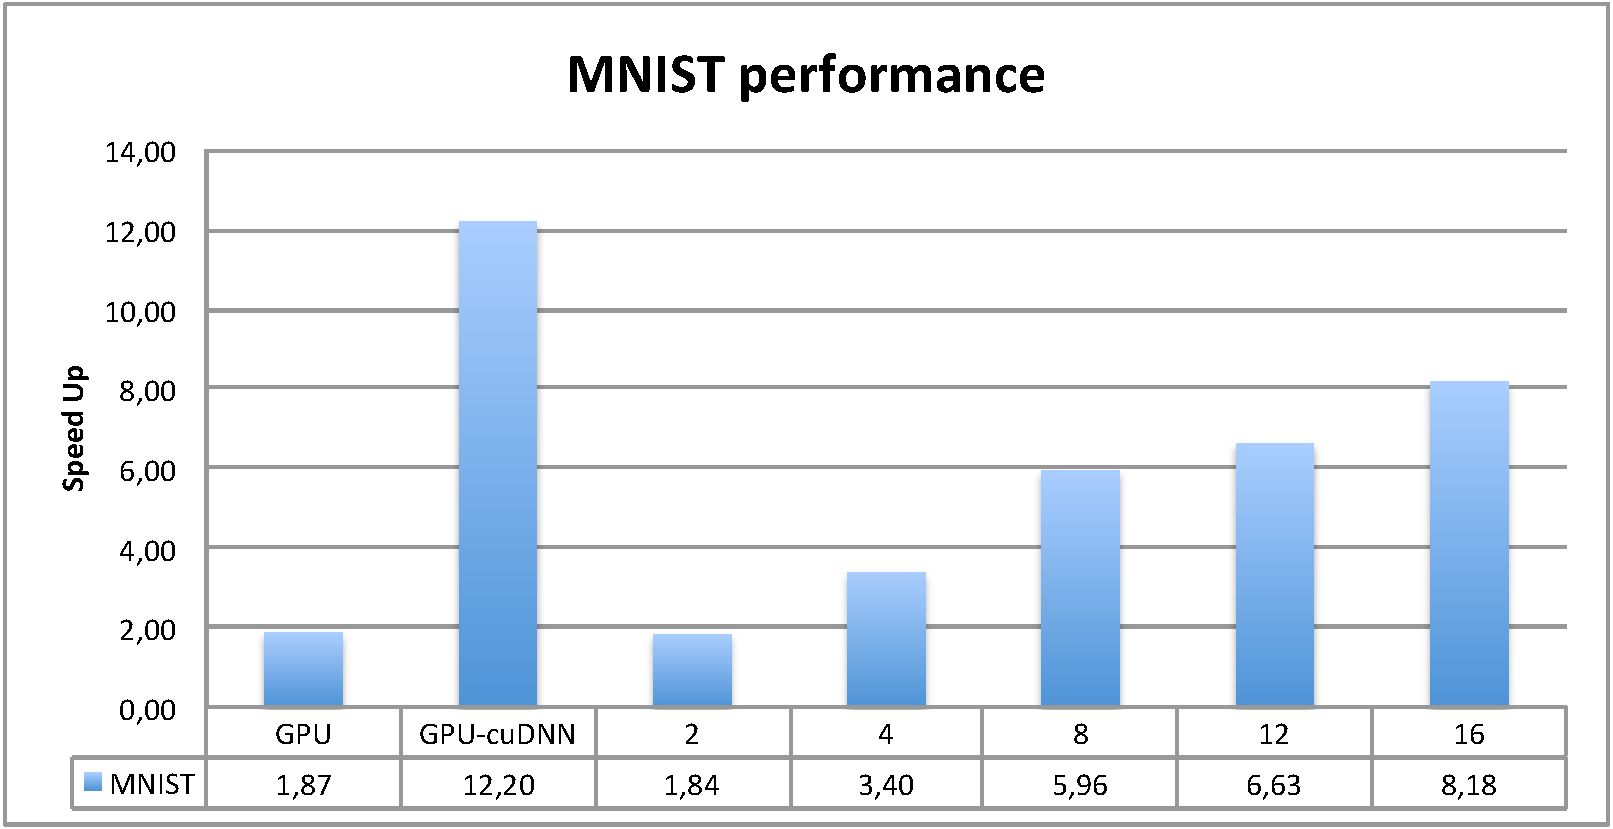
\includegraphics[width=\linewidth]{figures/mnist-abs-perf-all.pdf}
\caption{\todo{CAPTION}}
\end{figure}

%\begin{figure*}[]
%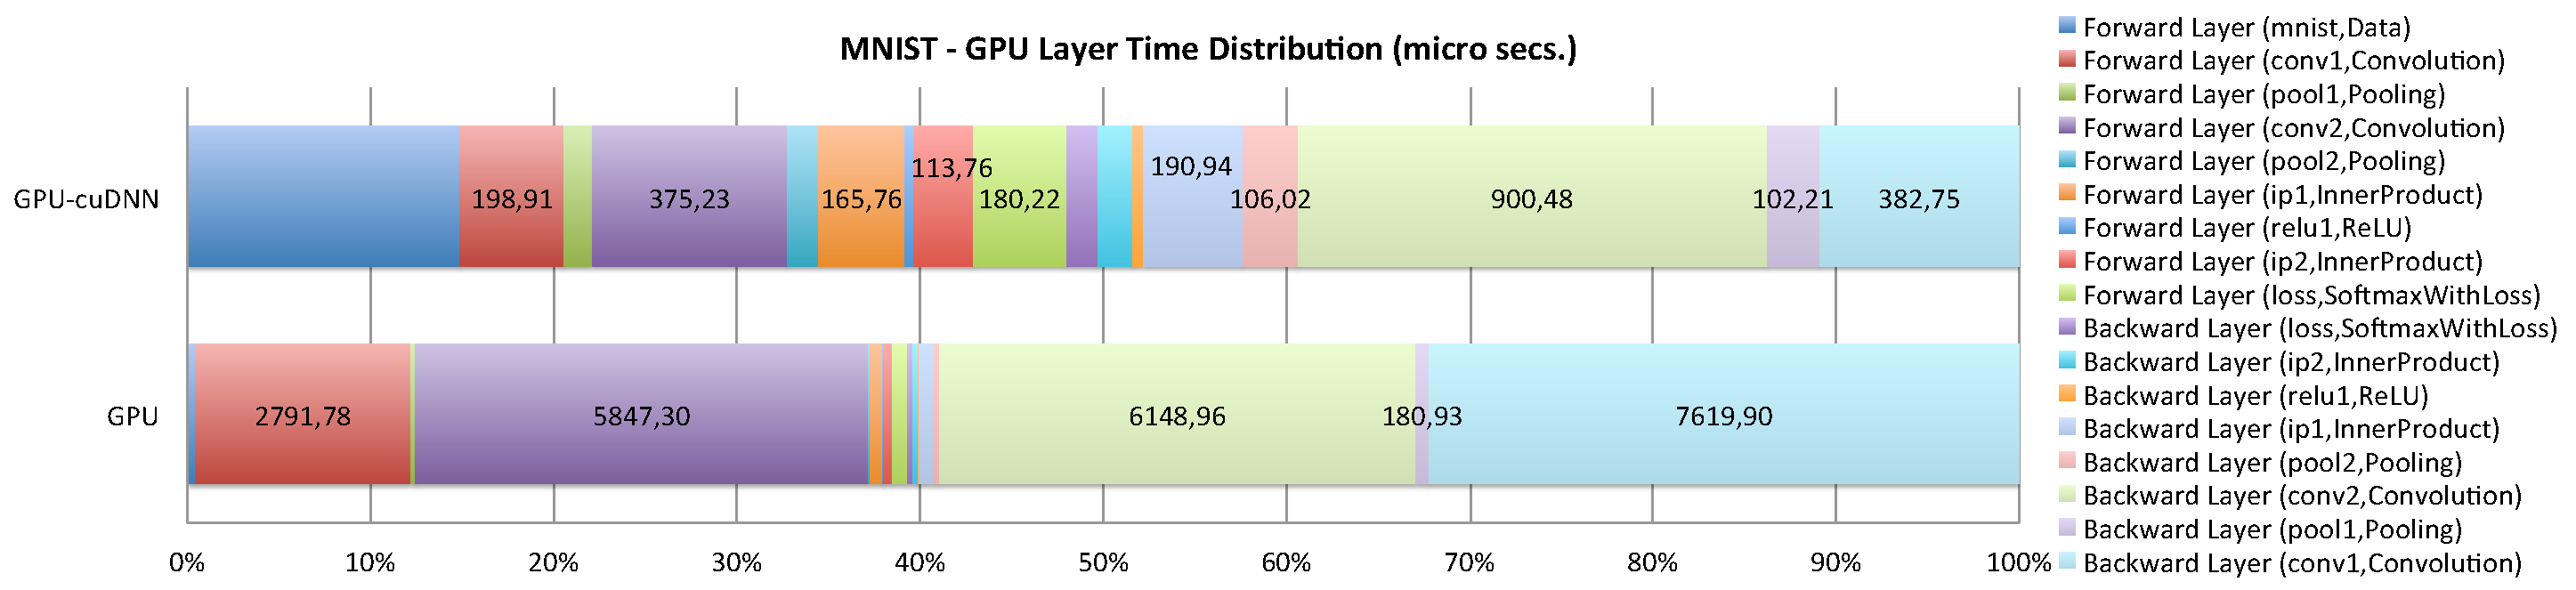
\includegraphics[width=\linewidth]{figures/mnist-gpu-rel-abs-time.pdf}
%\caption{\todo{CAPTION}}
%\end{figure*}

\begin{figure}[]
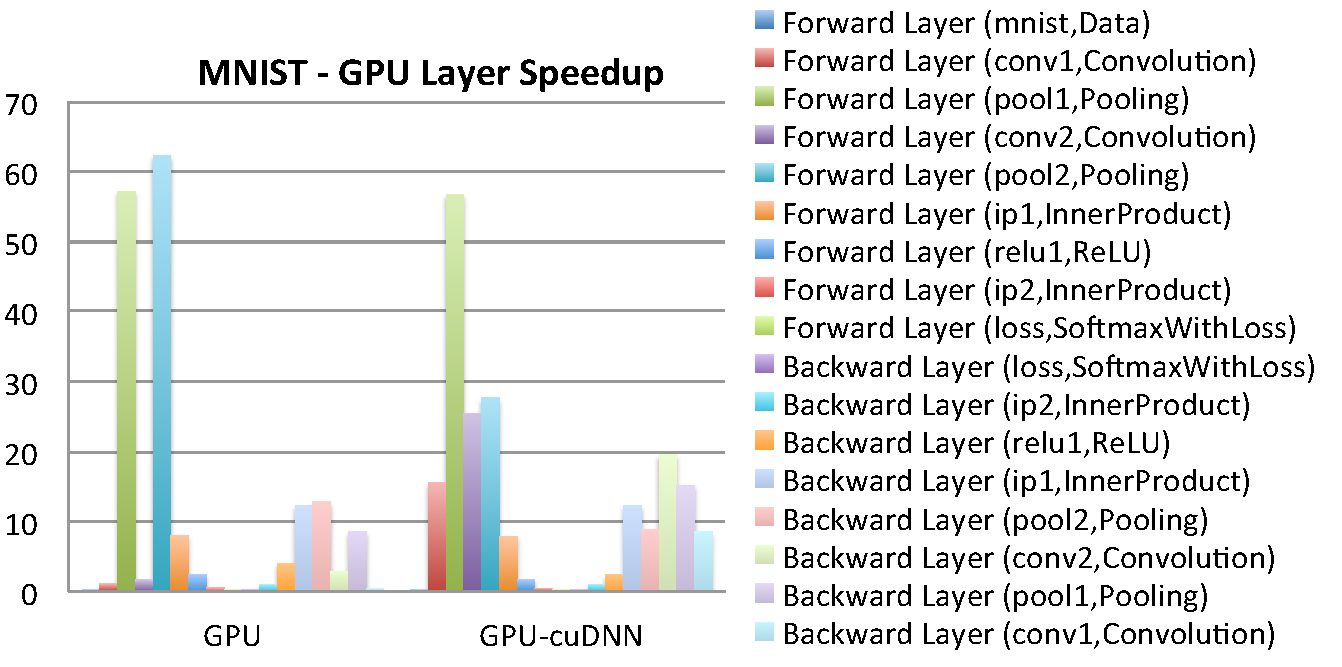
\includegraphics[width=\linewidth]{figures/mnist-gpu-layer-speedup.pdf}
\caption{\todo{CAPTION}}
\end{figure}

\subsection{Performance Limiting Factors}
We have identified several factors that affect the batch-level
parallelization of the Caffe DNN framework. These factors are
layer dependant and are mainly related to specificities of the
layers that determine their work distribution, memory footprint,
data privatization and ordered operations. The following subsec-
tions describe these limiting factors.

\textbf{Sequential memory allocation}: the network memory allocation
happens during the network initialization. This process is sequen-
tial, which causes the layer memory be allocated following a
pattern generated by the initialization code. In terms of perfor-
mance, this pattern is not compatible with those that arise during
the training process.

\textbf{Locality between layers:} the input/output relation across layers
defines a lost of data locality for specific layers. During the for-
ward and backward phases, each layer distributes the work ac-
cording to the dimensions of the input blobs. Regarding the data
locality, it is possible that input and output blobs do not match
their dimensions. Consequently, the work distribution and thread-
data association defined in one layer will not match that one of the
next immediate layer in the stack, causing some data movement
across the memory hierarchy.

One particular case of this situation corresponds to the data
layers in Caffe. These layers feed the network with input data
organized in batches. Data layers execute in single-thread mode.
Therefore, a one thread first accesses all data and then the data is
distributed across the cores and the memory hierarchy when the
first parallel processing layer in the network is executes in paral-
lel. 

\textbf{Work unbalance:} coarse grain parallelism is open to work unbal-
ance. For the Caffe case, we have detected that batch-level paral-
lelism defines very heavy iterations for the parallelized loops.
Therefore, one single loop iteration can cause a high unbalance
between the executing threads. In general, threads receive the
same number of iterations (e.g.: under a static scheduling). But it
is possible that some of the threads receive one more iteration
than other threads when the number of samples in the batch is not

\textbf{Work granularity:} as previously described, neural networks try
to perform a dimensionality reduction over the processed data.
And this affects the size of the working sets in the network layers.
At some level in the network, the input/output blobs start decreasing their sizes. When this happens, a thread level parallelization
starts suffering from too small work granularity with poor performance levels.

\textbf{Data privatization and reduction operations:} specifically in the
backward phase, the network coefficients are updated per each
sample in the batch. At batch-level, this requires mutual exclusion
mechanisms to guarantee a correct update. Data privatization has
been needed for this purpose. Caffe is implemented following an
object-oriented design and object privatization (e.g.: blobs) has
performance implications regarding the invocation of object constructor/destructor.

\subsection{The MNIST case}
\todo{Brief paragraph summarizing methodology.}

\subsubsection{Layer Performance}
\todo{Figure XXX-abs-time} shows relative weight in the overall execution time and absolute execution time numbers for all layers in the
MNIST network. The absolute values correspond to 100 training
iterations where every iteration processes a batch of 64 images.
The immediate observation is that two layers dominate the execution time training execution: the convolution and pooling layers.
Both for their forward and backward phases account for almost
65\% of the execution time.

\todo{Figure XXX-speedup} shows the scalability numbers for all
layers. In general, we observe three behaviours. Some layers do
not respond to the increment of threads in both the forward and
backward phases (data series below the 3 value in Figure XXX-
speedup). This is directly related to the size of input and output
blobs and the granularity of the computation. Other layers expose
a poor scalability, with speed up numbers between 2 and 6. For
these layers, data locality is the main cause for their low performance. It happens that input and output blobs between two immediate layers have very different shapes. The work distribution for
threads is determined according to the input blob shape. Therefore, two consecutive layers will have different work distribution
with the associated data movement across the memory hierarchy.
Finally, layers with reasonable scalability correspond to layers
heavily weighted in computation. Besides, these layers share a
common blob shape between their immediate layers in the stack.
The following subsections give detail of every layer in the MNIST
network in terms of absolute execution time, scalability curves
and the main factors that limit their performance.
\todo{Mention that with more than 8 threads, the serial network initialization makes suboptimal the utilization of the memory nodes. Is
there any HW counter we could measure to show this?}

\textbf{mnist (Data Layer):} this corresponds to the layer responsible for
feeding the network with data samples. The layer reads from disk
64 images from an image database. In order to overlap this IO
operation, the data layer operates with a pre-fetching thread that
brings data enough in advance so that the network training never
is stopped waiting for the IO to complete. The layer executes
sequentially and has very small weight in the overall execution
time. Nevertheless, because its sequential execution, it affects the
performance of the immediate layer in the network, the convolutional layer conv1.

\textbf{conv1 (Convolutional Layer):} the conv1 layer is affected by a
poor data locality given the serial execution of its immediate
previous data layer. The layer is not affected by work balance
issues as the batch size is 64, so for 2, 4, 8 and 16 threads, all
threads process the same number of data samples. The forward
layer phase, it represents a relative small part of the execution
time (7\% of the execution time no matter the number of threads,
see \todo{Figure XXX}). But this phase includes sufficient work to benefit form the batch-level parallelism. \todo{Its blob input and output sizes
are XXX and XXX respectively}. Its scalability curve shows
speedups of 1.85, 3.43, 6.57 and 10.94. The effect of the data
locality can be seen when compared to a layer of the same type
but in an inner level of the network. The conv2 layer shows a
better scalability (see the explanations below). \todo{The conv1 backward phase exposes similar trends and is affected by reduction
and data privatization overheads.}

pool1 (Pooling Layer): this layer follows the same work distribu-
tion scheme as the conv1 and conv2 layer, so no data locality nor
work distribution issues are present along its execution. The input
and output blobs are read/written exactly in the same manner they
are produced by the immediate neighbouring layers. The forward
layer phase corresponds to a 6\% of the execution time with input
and output blob sizes of \todo{XXX and XXX} respectively. In terms of
scalability, this phase presents speed up numbers of 1.83, 3.43,
6.13, and 10.94 with 2, 4, 8, and 16 threads respectively. The
backward phase corresponds to a 2\% of the execution time with
speed up numbers of 2.18, 3.96, 7.64, and 9.69 for 2, 4, 8 and 16
threads respectively.

\textbf{conv2 (Convolutional Layer):} this layer shows very similar
trends as the conv1 layer. It does not suffer from any locality issue
with its immediate previous pool1 layer. It is more computationally 
intensive than conv1, as its parameters define larger input and
output blobs (\todo{XXX and XXX} respectively). The forward phase
corresponds to 20\% of total execution time no matter the number
of threads. It shows a curve of scalability with speed up numbers
of 1.93, 3.58, 6.64 and 13.12 with 2, 4, 8 and 16 threads respectively. The backward phase is much computationally significant
as it corresponds to almost 40\% of the serial execution time, but
decreasing its contribution as the number of threads increases.
This is explained by the fact that other layers with worst scalability curves become more dominant of the overall execution time.

\textbf{Pool2 (Pooling Layer):} this layer experiments a mismatch in
terms of work and data distribution with its immediate neighbour
layer ip1. This determines a very poor scalability with more than 8
threads. The pool2 and ip1 layers operate with very different blob
shapes. The pool2 layer is parallelized according to its input blob
structure. This causes the output blob (input blob for ip1) to be
generated by threads that later in the ip1 layer will be assigned
with different working sets. Thus, causing data movement across
the memory hierarchy. The forward layer phase corresponds to a
3\% of the execution time with input and output blob sizes of XXX
and XXX respectively. In terms of scalability, this phase presents
speed up numbers of 1.59, 2.83, 5.52, and 4.94 with 2, 4, 8, and
16 threads respectively. The backward phase corresponds to a 2\%
of the execution time with speed up numbers of 1.71, 3.23, 5.73,
and 2.56 for 2, 4, 8 and 16 threads respectively. In addition, the
backward phase is affected by a small granularity in its backward
phase.

\textbf{ip1 (Inner Product Layer):} this layer is affected by a poor data
locality with the previous pooling layer pool2 (see above). The
scalability curve is poor when more than 8 threads are used. The
forward phase presents speedup numbers of 1.75, 3.19, 4.58 and
4.83 with 2, 4, 8 and 16 threads respectively. It corresponds to
about 2\% of the execution time in any thread configuration. The
backward phase exposes a similar trend with speed up numbers of
1.83, 2.38, 5.93 and 5.79. It corresponds to about 5\% of the execution time.

\textbf{Relu (Relu Layer), Ip2 (Inner Product Layer), Loss (Softmaxwithloss Layer):} these layers are totally conditioned by the
sizes of their input/output blobs and their work granularity. In
general, the work here is too small for experiencing any im-
provement from a parallel execution. These layers correspond to
the inner most layers in the network, where all the dimensionality
reduction has been applied. For instance, the Relu layer generates
a blob of only 500 elements; or the ip2 layer generates an output
blob of just 10 elements (one per image class). This happens for
both the forward and backward phases.

\subsubsection{Overall Performance}
\todo{Figure XXX-overall-speedup} shows the overall performance of
the GPU and the CPU coarse-grain parallelization. The CPU
version reaches close to a 6x speedup with 8 threads, and 8x with
16 threads. The lack of the scalability for the CPU version is
related to the poor scalability of fine-grained layers that when
executing with 16 threads drag down the performance. Also, we
suspect the serial initialization of the network is giving a suboptimal memory allocation in the NUMA nodes. All of this is affecting the final scalability of the CPU version. In contrast, the GPU
version shows a modest speed up close to 2x. The reason for this
difference is related to the performance of the convolutional layers.

\todo{Figure XXX-percentage-GPU} shows the computational contribution of each layer and \todo{Figure XXX-GPU-speedups} shows the
speed up for each layer. The layer dominance is completely the
same as in the CPU version. And the GPU gives extraordinary
speed ups for the pooling layers. All other layers expose speedup
similar to those obtained by the CPU version, unless the convolution layers. They dominate the overall execution and suffer from
very poor speedup. The cuDNN version solves this issue with the
usage of parallel GPU streams enabling the execution of several
convolutions simultaneously, plus a highly optimized convolution
implementation. ADRESS the NO GENERALITY OF CUDNN.
\todo{The case of cuDNN and its extraordinary performance is addressed in section XXX.}

\subsection{The CIFAR-10 case}

The dataset is divided into five training batches and one test batch, each with 10000 images. The test batch contains exactly 1000 randomly-selected images from each class. The training batches contain the remaining images in random order, but some training batches may contain more images from one class than another. Between them, the training batches contain exactly 5000 images from each class. 
\subsubsection{Layer Performance}
\todo{Similar as MNIST}

\subsubsection{Overall Performance}
\todo{Similar as MNIST}

\subsection{Caffe and cuDNN}
\todo{- In 2012, Caffe won the ILSVRC2012-winning SuperVision
model and caching IO.
- CPU version is not comparable in terms of the optimization
efforts.
- cuDNN is not general enough, it is totally oriented to image
classification NO GENERALITY. Main success for accelera-
tion of convolutions reaching speedups of XXXX.
Make an example: no current support for LSTM in cuDNN,
other examples ??
Build the case for cuDNN NOT being a general framework for
DNN.
Compare with GPU BLAS level approach (and GPU-cuDNN?)
}



